\documentclass[11pt,a4paper]{article}

\usepackage[margin=2.5cm]{geometry}
\usepackage{amsmath}
\usepackage{amssymb}
\usepackage{booktabs}
\usepackage{array}
\usepackage{ragged2e}
\usepackage{seqsplit}
\usepackage{enumitem}
\usepackage{xcolor}
\usepackage{listings}
\usepackage[hidelinks]{hyperref}
\usepackage{caption}

%--------------------------
%  GRAPHICS / FIGURES
%--------------------------
\usepackage{float}
\usepackage{graphicx}

\DeclareGraphicsExtensions{.png}
\graphicspath{{figs/}}

\newcommand{\file}[1]{\texttt{\seqsplit{#1}}}
\newcommand{\code}[1]{\texttt{#1}}
\newcommand{\erf}{\operatorname{erf}}
\setlength{\emergencystretch}{3em}
\newcolumntype{L}[1]{>{\RaggedRight\arraybackslash}p{#1}}

\definecolor{codebg}{gray}{0.96}
\lstdefinestyle{py}{
  language=Python,
  basicstyle=\ttfamily\footnotesize,
  backgroundcolor=\color{codebg},
  frame=single,
  numbers=left,
  numberstyle=\tiny\color{gray},
  breaklines=true,
  breakatwhitespace=true,
  showstringspaces=false,
  keywordstyle=\color{blue!55!black},
  commentstyle=\color{green!35!black},
  stringstyle=\color{red!45!black},
  captionpos=b,
}

\title{Characterizing the Dark Signal\\
\large Six tests, in order, and the two decisions they led to}
\author{Colorimeter project --- pad analysis pipeline}
\date{Generated 2026-09-11 against branch \file{preimage-capture}}

\begin{document}
\maketitle

\begin{abstract}
\noindent
Every measurement this instrument makes starts by subtracting a ``dark''
exposure --- a frame read out with no light reaching the sensor --- from the
corresponding lit frame, on the reasoning that whatever the sensor reports
with no light present is an offset to be removed, not signal. Until now that
subtraction has never been examined on its own: we always looked at it as
part of the larger reflectance calculation. This document works through six
increasingly specific questions about the dark signal, each posed in plain
language, answered with an explicit and elementary statistical method, and
illustrated with a figure produced by
\file{desktop/padanalysis/analysis\_2.py}. The questions build on one
another: is a single dark frame just noise, or does it have structure; if it
has structure, is that structure the same pixel to pixel and stable over
time; does it drift; does it depend on how long the exposure was; and,
putting all of that together, what is actually the best thing to subtract
from a future lit frame. Two practical decisions follow directly from the
answers, and both are stated at the end: subtract a fresh dark frame's own
average level rather than its raw pixel-by-pixel values, except at a small,
explicitly identified set of pixels that behave differently; and replace the
present ladder of many exposure times with a pair of ``before'' and
``after'' dark batches, since the dark level turns out not to depend on
exposure duration by an amount worth chasing.
\end{abstract}

\tableofcontents
\newpage

%======================================================================
\section{Introduction and scope}
%======================================================================

\subsection{Why this document exists}

The photometric chain used elsewhere in this project (see
\file{tex/R\_inf\_guide.tex}) begins with \code{sig = lit - dark}: every
downstream quantity, from the raw ratio \code{R} through \code{A} and
\code{K/S}, inherits whatever error is in that one subtraction. Nobody had
asked, with real data and a real method, how good that subtraction actually
is, or whether it could be made better cheaply. This document is the record
of asking. It follows the ``show the method, not just the answer'' habit
already established for this project's analysis notes: each section states
why a question mattered, what test was chosen to answer it, how that test
was implemented, and what the result actually was --- including where a
result surprised us or needed a second look.

\subsection{What data this is based on}

Every number and figure below comes from nine archives, \code{C1017}
through \code{C1025}, read through channel \code{B} (one of the four Bayer
layers; see \S\ref{sec:notation}) of the measurement sweep. Two of the nine
(\code{C1017}, \code{C1018}) are ``exposure-ladder'' captures that took a
dark frame at 22 different exposure times; the remaining seven took a dark
frame at 8 exposure times each. Pooled, this gives 100 stored dark frames,
each $130 \times 183$ pixels (23{,}790 pixels) in the bound-crop layer grid
this project works in. This is a convenience sample, not a designed
experiment --- it is what happened to be captured for an unrelated purpose
(the round-dot dye series) --- and every conclusion below should be read
with that in mind. Two limitations are worth stating up front rather than
discovering later: everything here is channel \code{B} only, and every dark
frame used is an ``after'' frame (see \S\ref{sec:decisions}); the older
``before/after'' pairing this document ultimately recommends reinstating is
not itself present in this sample.

\subsection{Where the code lives}

Every function named below is in \file{desktop/padanalysis/analysis\_2.py}.
It is read-only against the archives and writes nothing but figures, so
every result here can be reproduced by calling the named function with the
same sample list.

%======================================================================
\section{Notation and terms}
\label{sec:notation}
%======================================================================

Some of this is camera terminology, some is statistics terminology. Both
are defined here once, and used consistently afterward.

\subsection{The data}

\begin{description}[leftmargin=2.2cm,style=nextline]
\item[DN] ``Digital number,'' the raw unit a pixel is read out in. This
  sensor's analog-to-digital converter is 10-bit, so a single raw reading is
  an integer from 0 to 1023.
\item[Bayer layer] A color camera sensor covers its pixels with a repeating
  $2\times2$ pattern of color filters: one red, one blue, and two green
  (traditionally called \code{Gr}, the green filter sharing a row with red,
  and \code{Gb}, the green filter sharing a row with blue). This project
  treats the four as four separate images, called \emph{layers}, each at
  half the sensor's linear resolution. \S\ref{sec:notation} onward writes
  $\mathrm{ch} \in \{R, Gr, Gb, B\}$ for which layer, and every result in
  this document uses $\mathrm{ch} = B$.
\item[Bound-crop layer grid] The small rectangular region of one layer that
  actually contains the test strip, in that layer's own row/column
  coordinates. For this sample set it is $130$ rows by $183$ columns, i.e.\
  $N_{\mathrm{px}} = 23{,}790$ pixels.
\item[Exposure] How long the sensor integrates light (or, for a dark frame,
  how long it integrates nothing) before being read out, in microseconds
  ($\mu s$). One archive stores one dark frame per distinct exposure time
  used anywhere in its lit sweep; ten LEDs sharing the same exposure time
  share that one dark frame (\file{probe.py}, \code{Capture.\_dark\_link}).
\item[Archive / sample] One capture, e.g.\ \code{C1017}, stored as one HDF5
  file. Everything in this document uses the ``measurement'' section of the
  archive (as opposed to the shorter ``pre-image'' section; see
  \file{probe.py}'s module docstring).
\item[Pixel index $i$] A single location in the bound-crop layer grid.
  Where a formula sums or averages ``over $i$,'' it means over all
  $N_{\mathrm{px}}$ pixels of that grid.
\item[Frame index $k$] One particular stored dark frame, $k = 1, \dots, n$,
  where $n$ is however many dark frames a given calculation pools together
  (e.g.\ $n = 100$ for the nine-archive pool used throughout this document).
  Do not confuse $n$ (a count of frames) with $N_{\mathrm{px}}$ (a count of
  pixels) --- both appear in the same formulas below.
\item[$d_i(k)$] The dark-subtracted-nothing, i.e.\ raw, reading of pixel $i$
  in frame $k$, in DN. This is what \code{probe.Capture.darklayer} returns.
\end{description}

\subsection{The statistics}

Each of these is also introduced again, briefly, the first time it is used;
this is a single place to look them back up.

\begin{description}[leftmargin=2.2cm,style=nextline]
\item[Mean, variance, standard deviation] For a list of $M$ numbers $x_1,
  \dots, x_M$: the mean is $\bar{x} = \frac{1}{M}\sum_j x_j$; the variance
  is $\mathrm{Var}(x) = \frac{1}{M-1}\sum_j (x_j - \bar x)^2$ (dividing by
  $M-1$ rather than $M$ is the small, standard correction that makes this
  an unbiased estimate of the true population variance when $\bar x$ itself
  was estimated from the same data); the standard deviation $\sigma$ is the
  square root of the variance, in the same units as the data.
\item[Pearson correlation coefficient, $r$] For two paired lists $a_j,
  b_j$, $r = \mathrm{cov}(a,b) / (\sigma_a \sigma_b)$, where
  $\mathrm{cov}(a,b) = \frac{1}{M-1}\sum_j (a_j - \bar a)(b_j - \bar b)$.
  $r$ ranges from $-1$ to $1$; $r^2$ is the fraction of one list's variance
  that is shared with (linearly predictable from) the other.
\item[Empirical cumulative distribution function (CDF)] For $N$ sorted
  values $x_{(1)} \le x_{(2)} \le \dots \le x_{(N)}$, the empirical CDF at
  $x_{(i)}$ is $F_{\mathrm{emp}}(x_{(i)}) = (i - \tfrac12)/N$: the fraction
  of the data at or below that value. It is the data's own answer to ``what
  fraction of values are this small or smaller.''
\item[Normal (Gaussian) distribution and $\erf$] The familiar bell curve
  with mean $\mu$ and standard deviation $\sigma$. Its CDF has a closed
  form written in terms of the error function, $\erf(z) = \frac{2}{\sqrt\pi}
  \int_0^z e^{-t^2}\,dt$: $F_{\mathrm{normal}}(x) = \frac12\left[1 +
  \erf\!\left(\frac{x - \mu}{\sigma\sqrt2}\right)\right]$.
\item[Permutation test] A way to ask ``is this pattern more than I would
  see from shuffled, meaningless data,'' without assuming the data are
  normally distributed. Compute the statistic of interest on the real data;
  then shuffle the labels (e.g.\ which exposure or which time each value is
  attached to) many times, recomputing the same statistic each time, to
  build up a distribution of what the statistic looks like when there is,
  by construction, no real relationship. The fraction of shuffled trials
  whose statistic is at least as extreme as the real one is the
  (Monte Carlo) $p$-value.
\item[One-way ANOVA and the $F$-statistic] A way to ask whether several
  groups of numbers have different means, given only how spread out each
  group is internally. Defined and derived where first used,
  \S\ref{sec:exposure}.
\item[Statistical vs.\ practical significance] A result can be
  statistically detectable (unlikely to be pure chance) while still being
  too small to matter for any practical purpose. Both a $p$-value and an
  effect size (how big the difference actually is, in DN) are reported
  together below for exactly this reason.
\end{description}

%======================================================================
\section{A first look at one dark frame}
\label{sec:first-look}
%======================================================================

\paragraph{Why we asked this.}
Before any statistics, the most basic question is simply: what does a dark
frame look like? Is it visually uniform, or does it have obvious structure?
What is a typical value, and how much do pixels vary around it?

\paragraph{What we did.}
\code{dark\_analysis1(samp\_no, exposure\_ms, ch)} reads one dark frame
through \code{probe.Capture.darklayer} and draws it two ways side by side:
as an image, and as the same pixel values sorted from darkest to brightest
($d_{(1)} \le d_{(2)} \le \dots \le d_{(N_{\mathrm{px}})}$). The sorted view
turns 23{,}790 numbers into one line: a flat middle with short ramps at
each end is ordinary noise sitting on a uniform offset; a long slope, a
step, or an isolated jump at either end is something structural --- a hot
pixel at the top, a cold or dead one at the bottom.

\paragraph{What we found.}
Figure~\ref{fig:single-frame} shows one dark frame from \code{C1017} at a
$50.973\,\mathrm{ms}$ exposure. Two things stand out, and both matter for
everything that follows. First, the frame looks like ordinary speckle: no
visible large-scale pattern, no obviously distinct pixels beyond a handful
of very faint bright specks. Second, and easy to miss: the sorted curve on
the right is a \emph{staircase} with only five steps, at 62, 63, 64, 65, and
66~DN. A single raw dark reading is a 10-bit integer, and with a mean near
64~DN and a spread of well under one DN, the entire 23{,}790-pixel frame
only occupies about five integer values. This is not a defect; it is simply
the resolution of one raw reading, and it becomes important again in
\S\ref{sec:normality}, where it explains a pattern that could otherwise be
mistaken for something more interesting.

\begin{figure}[H]
\centering
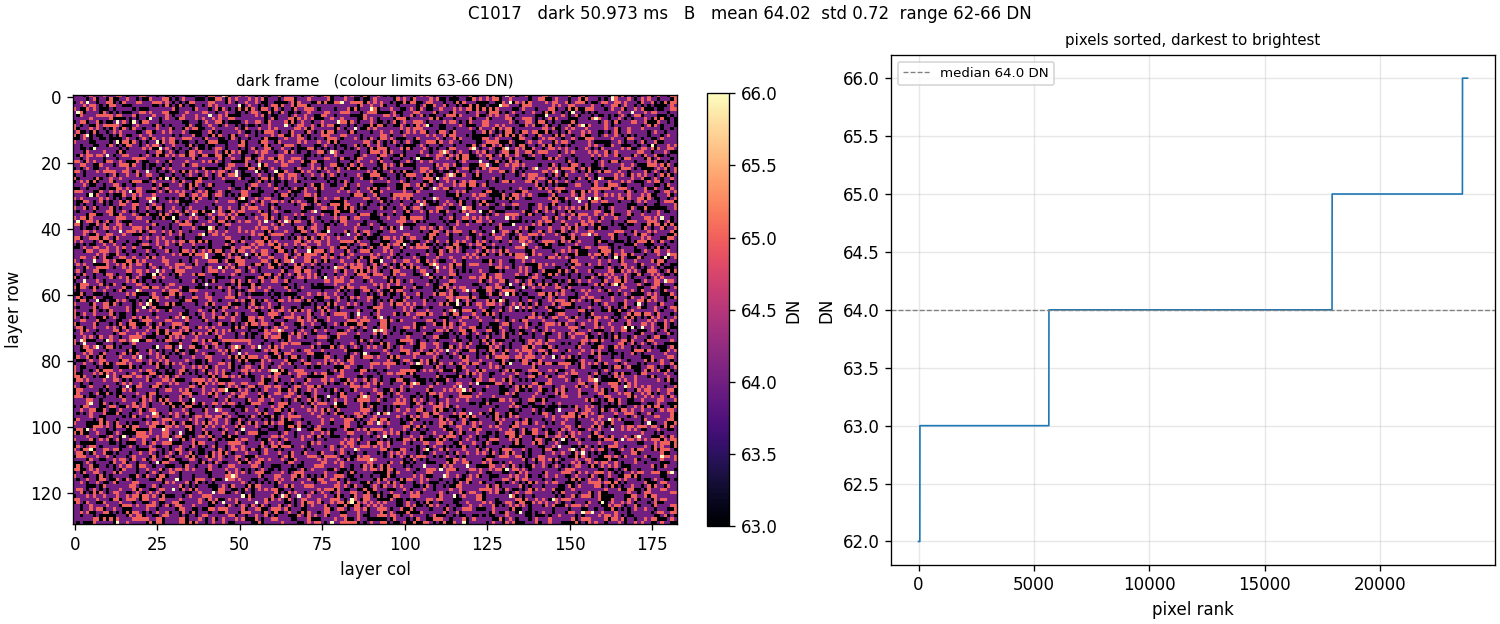
\includegraphics[width=\linewidth]{dark-signals-single-frame}
\caption{One raw dark frame, \code{C1017}, exposure $50.973\,\mathrm{ms}$,
channel \code{B}. Left: the frame as an image. Right: the same 23{,}790
pixel values sorted from darkest to brightest --- note the staircase, a
direct consequence of the sensor's 10-bit integer readout.}
\label{fig:single-frame}
\end{figure}

%======================================================================
\section{Is there a real pixel-to-pixel pattern, or is it all noise?}
\label{sec:model}
%======================================================================

\paragraph{Why we asked this.}
One frame cannot answer this. A pixel that reads a little high in one frame
might just be having a noisy moment; only by looking at the same pixel
across many frames can ``consistently a little high'' be told apart from
``high just this once.''

\paragraph{The model.}
We adopt the simplest structure that lets that question be asked at all:
for pixel $i$ in frame $k$,
\begin{equation}
d_i(k) \;=\; \mu(k) \;+\; p_i \;+\; \varepsilon_i(k),
\label{eq:model}
\end{equation}
where
\begin{itemize}
\item $\mu(k)$ is frame $k$'s own \emph{spatial mean} --- the average of
  $d_i(k)$ over all pixels $i$ in that one frame. It is a property of the
  frame, not of any pixel, and it is the term that can drift with time or
  with exposure (\S\ref{sec:temporal}, \S\ref{sec:exposure}).
\item $p_i$ is pixel $i$'s own fixed, time-invariant offset from the frame
  mean --- the ``fixed pattern.'' If $p_i$ is a real, reproducible property
  of the pixel, it should look the same no matter which frames are used to
  estimate it; \S\ref{sec:stability} tests exactly that.
\item $\varepsilon_i(k)$ is whatever is left over: fresh, independent noise,
  one new random draw for this pixel in this frame, uncorrelated with
  $p_i$ and with $\varepsilon_i$ in any other frame. (Earlier work on this
  project established that $\varepsilon_i(k)$ is also spatially
  independent --- knowing one pixel's noise says nothing about its
  neighbor's --- so nothing here needs to borrow strength across
  neighboring pixels.)
\end{itemize}
This is nothing more than ``every reading is a frame-level average, plus a
personal bias for this pixel, plus leftover noise'' written as an equation.
Everything from here on is about estimating the three pieces on the right
separately, because they behave differently and, as \S\ref{sec:estimator}
shows, deserve different treatment.

\paragraph{What we did.}
\code{dark\_analysis2(samps, ch)} stacks every stored dark frame for the
given samples and channel into one array, indexed by pixel and frame, and
computes two per-pixel summaries across the $n$ frames: the mean $\bar
d_i = \frac1n\sum_k d_i(k)$ and the standard deviation $s_i$ of $d_i(k)$
over $k$. Sorting pixels by $\bar d_i$ and plotting both quantities against
that sorted order is a direct visual test of Equation~\ref{eq:model}: if
$p_i$ were exactly zero for every pixel, the sorted-mean curve would be
flat (up to noise); if $\varepsilon_i(k)$ did not depend on the pixel's own
level, $s_i$ would also be flat across the sort.

\paragraph{What we found.}
Figure~\ref{fig:pixelstats} shows the result pooling all nine archives, $n
= 100$ frames. The top-left panel is the mean frame itself; on its own
percentile-based color scale it shows the same faint speckle as
Figure~\ref{fig:single-frame}, now averaged down to a much smaller range
(63.8--64.3~DN). The top-right panel is the telling one: the sorted mean is
very nearly flat across the great majority of pixels, climbing gently, but
rises sharply at the extreme right --- a small number of pixels sit clearly
above the rest, both in level and, in the bottom panels, in their own
standard deviation as well. Both bottom panels show the same thing at
different zoom levels: the noise level $s_i$ is essentially constant
(around $0.72$--$0.73\,\mathrm{DN}$) across the bulk of the population, and
only rises for that same handful of pixels at the far right. This is the
first evidence for a genuine, small population of ``hot'' pixels, distinct
from the ordinary noise floor --- a claim that \S\ref{sec:stability} tests
directly, rather than by eye.

\begin{figure}[H]
\centering
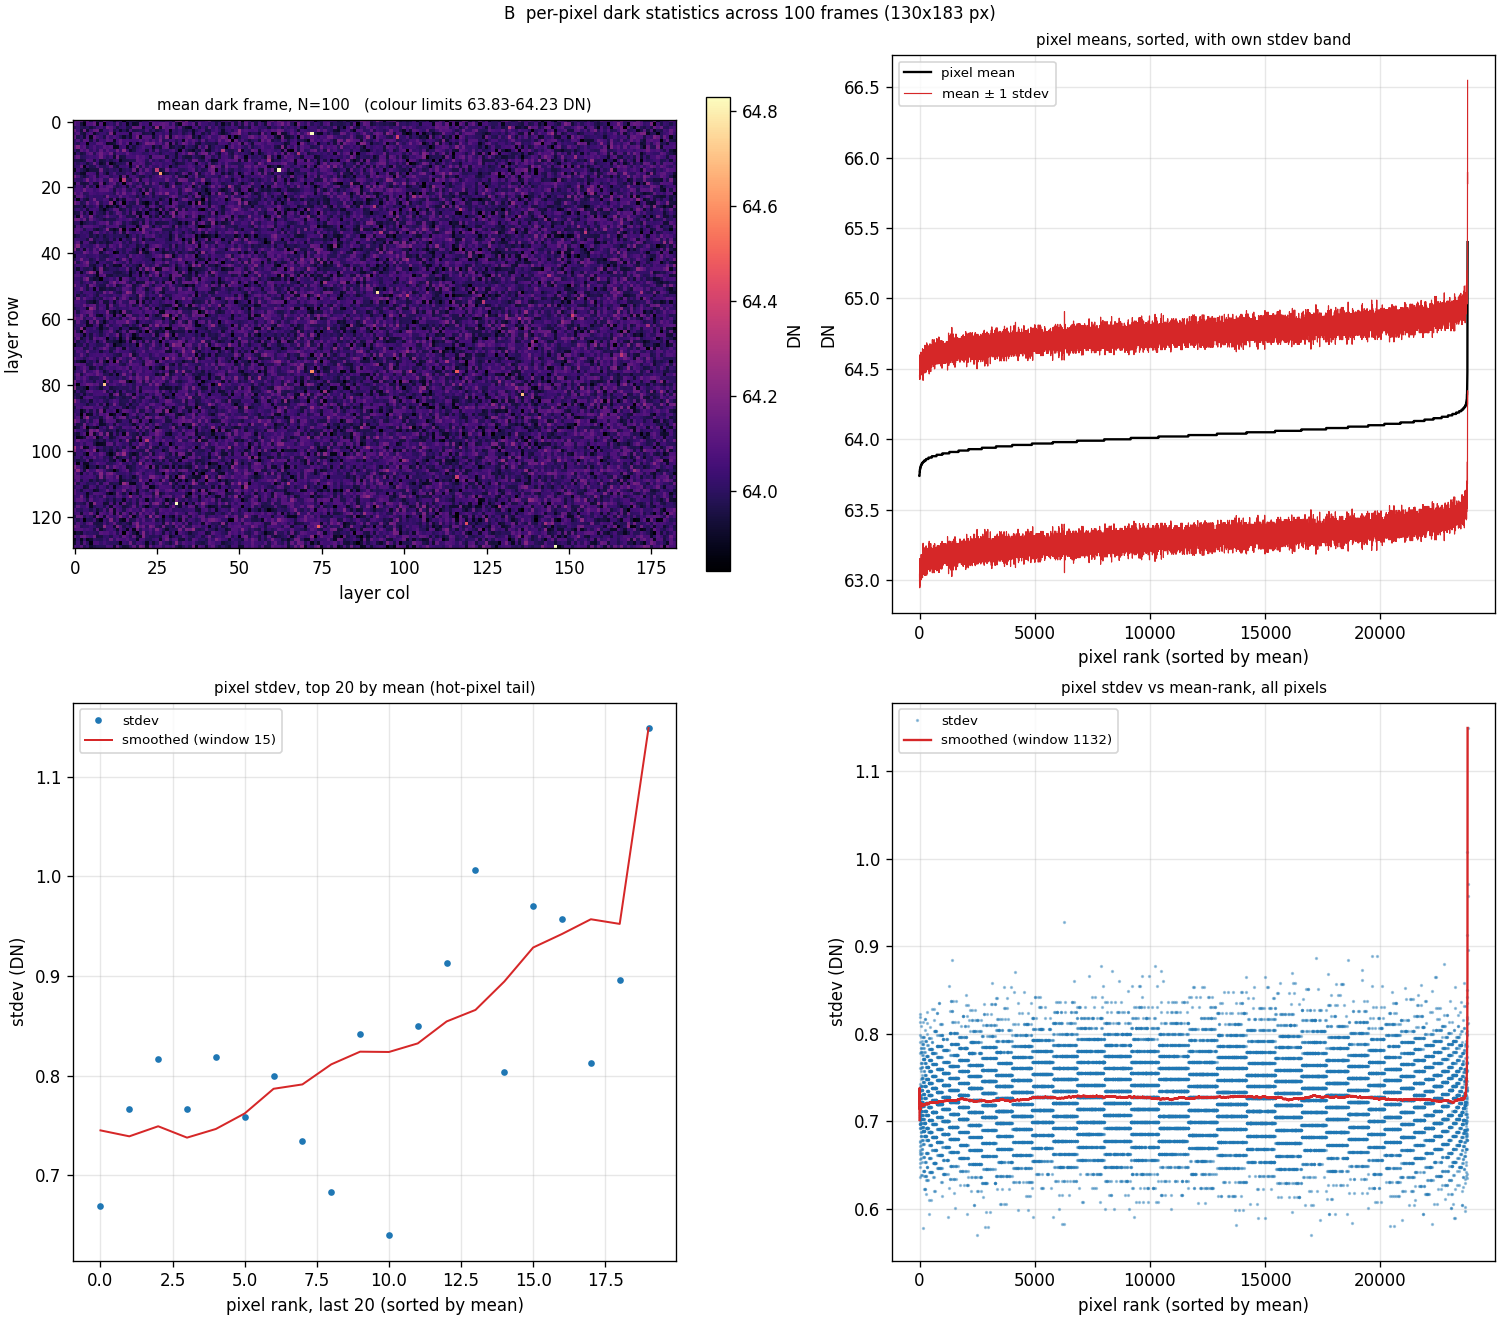
\includegraphics[width=\linewidth]{dark-signals-pixelstats}
\caption{Per-pixel dark statistics across all $n = 100$ pooled frames,
channel \code{B}. Top left: the mean frame. Top right: every pixel's mean
$\pm$ one of its own standard deviations, sorted by mean. Bottom: the same
per-pixel standard deviation, zoomed to the top 20 pixels by mean (left)
and shown for the whole population with two smoothing windows (right).}
\label{fig:pixelstats}
\end{figure}

%======================================================================
\section{Is the pixel-to-pixel pattern actually Gaussian noise?}
\label{sec:normality}
%======================================================================

\paragraph{Why we asked this.}
The sorted mean curve in Figure~\ref{fig:pixelstats} has the shape one
would expect if $\bar d_i$ were normally distributed across pixels ---
S-shaped when plotted this way is what a sorted sample of normal draws
looks like. But ``looks like'' is an eyeball judgment, and the estimator
built in \S\ref{sec:estimator} explicitly assumes $p_i$ is normally
distributed across the population of pixels. That assumption is worth
checking on its own terms, quantitatively, rather than taken on faith.

\paragraph{What we did.}
For a sorted sample $x_{(1)} \le \dots \le x_{(N)}$ (here, either the
per-pixel means or the per-pixel standard deviations from
\S\ref{sec:model}, with $N = N_{\mathrm{px}} = 23{,}790$), we compare the
empirical CDF defined in \S\ref{sec:notation} directly against the CDF of
the best-fitting normal distribution, using that same sample's own mean
$\hat\mu$ and standard deviation $\hat\sigma$:
\[
F_{\mathrm{emp}}(x_{(i)}) = \frac{i - \tfrac12}{N}, \qquad
F_{\mathrm{normal}}(x) = \frac12\left[1 + \erf\!\left(
\frac{x - \hat\mu}{\hat\sigma\sqrt2}\right)\right].
\]
Plotting both curves together is a direct visual test. Plotting their
difference, $F_{\mathrm{emp}} - F_{\mathrm{normal}}$, against $x$ makes the
same test quantitative: its largest magnitude anywhere is a
Kolmogorov--Smirnov-style distance, and, importantly, \emph{where} it
occurs says something about \emph{what kind} of deviation is present. This
is implemented in \code{dark\_cdf\_check(samps, ch, quantity)}, with
\code{quantity = "mean"} or \code{"std"} selecting which per-pixel
statistic is tested.

\paragraph{A caveat, stated rather than skipped.}
$\hat\mu$ and $\hat\sigma$ are estimated from the very sample being tested.
A more careful procedure (a Lilliefors test) accounts for the extra
flexibility this gives the fitted curve and uses a smaller, corrected
critical value than the textbook Kolmogorov threshold of
$1.36/\sqrt{N}$. We do not compute that correction here; the number below
should be read as a descriptive distance, not a calibrated $p$-value.

\paragraph{What we found --- and a correction to how we first read it.}
Figure~\ref{fig:cdfcheck} shows the check on the per-pixel mean. The two
CDFs agree closely almost everywhere; the maximum deviation is small,
$0.035$, at $x = 64.06\,\mathrm{DN}$. Our first pass at reading this kind of
plot assumed a deviation like this would sit in one tail and would mark the
hot-pixel population already seen in Figure~\ref{fig:pixelstats}. Looking
at the actual right-hand panel corrects that assumption: the deviation is
not a single bump in a tail but a rapid, symmetric zig-zag centered on the
\emph{bulk} of the distribution, near its mean, exactly where the data are
most dense. That shape has a specific, mundane explanation rather than a
statistical one: $\bar d_i$ is an average of $n$ ten-bit integers, so it can
only take values that are multiples of $1/n$; with $\hat\sigma$ of only
$0.078\,\mathrm{DN}$ (mean case) or $0.043\,\mathrm{DN}$ (standard-deviation
case), the whole distribution spans only a few dozen of those discrete
levels. A genuinely continuous normal distribution compared against data
that can only land on a comb of discrete values will always show exactly
this kind of oscillating deviation, largest where the data are densest, no
matter how large the sample gets. The hot-pixel evidence stands ---
Figures~\ref{fig:pixelstats} and~\ref{fig:stability} (next section) show it
directly --- but this particular figure is not where to look for it; it
mainly demonstrates that quantization, not a hot-pixel tail, is the
dominant departure from normality at the bulk of the distribution.

\begin{figure}[H]
\centering
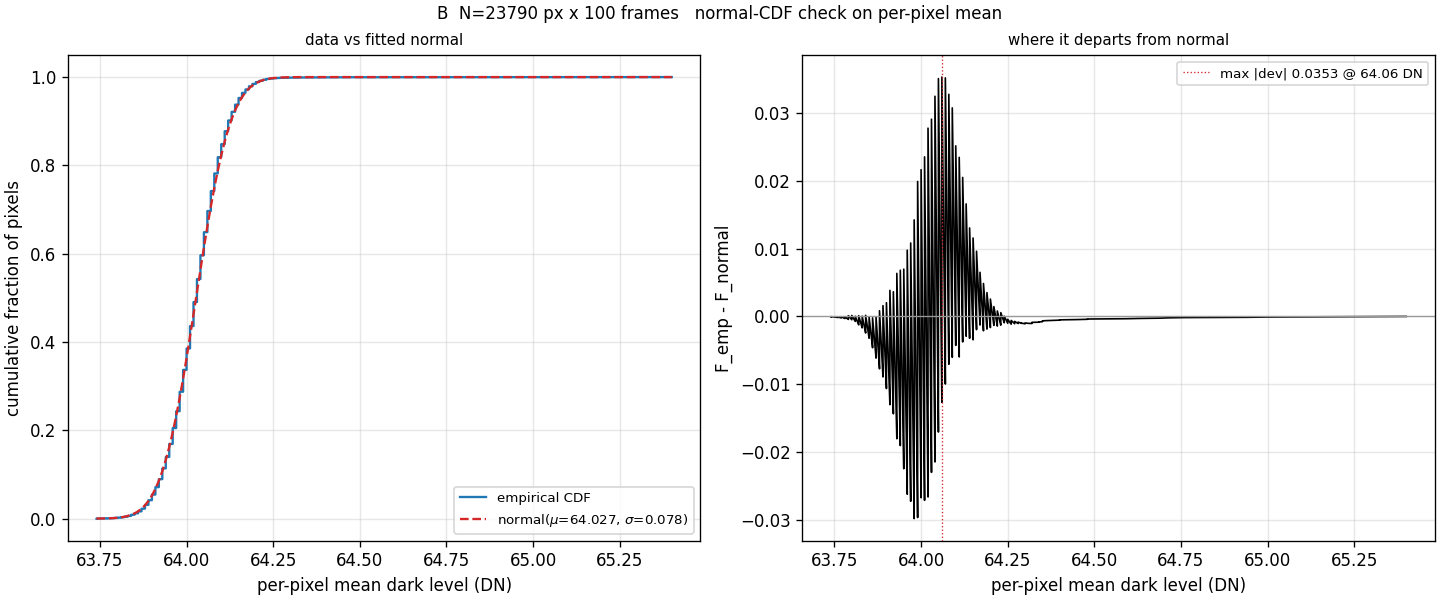
\includegraphics[width=\linewidth]{dark-signals-cdfcheck-mean}
\caption{Normal-CDF check on the per-pixel mean dark level, $n = 100$
frames, $N_{\mathrm{px}} = 23{,}790$ pixels. Left: empirical CDF against the
best-fit normal. Right: their difference. The rapid oscillation, centered
on the bulk rather than a tail, is a signature of the data's integer
quantization (\S\ref{sec:first-look}), not of a hot-pixel population.}
\label{fig:cdfcheck}
\end{figure}

%======================================================================
\section{Is the pattern stable over time, or just luck in this sample?}
\label{sec:stability}
%======================================================================

\paragraph{Why we asked this.}
A pixel could look ``hot'' in Figure~\ref{fig:pixelstats} purely by chance
--- with $100$ frames and $23{,}790$ pixels, some pixels will land at the
extreme of the distribution just from ordinary noise, the same way someone
in a large enough crowd will flip ten coins and get all heads. The only way
to tell a real, reproducible pixel property from a chance extreme is to
check whether it shows up again independently.

\paragraph{What we did: split-half reliability.}
This is a standard trick from measurement theory, elementary once stated:
split the available history into two independent halves (here, by time ---
the first $n/2$ frames and the last $n/2$), estimate each pixel's offset
separately in each half, and see how well the two independent estimates
agree. First remove the frame-level term using each frame's own spatial
mean, $r_i(k) = d_i(k) - \mu(k)$; a real, reproducible $p_i$ should agree
between the two halves; noise should not. Concretely, with $a_i$ the
average of $r_i(k)$ over the first half and $b_i$ the average over the
second half, the Pearson correlation $r = \mathrm{corr}(a, b)$
(\S\ref{sec:notation}) across all pixels is the fraction of each half's
variance that the two halves share --- i.e., the fraction that is a real,
stable property of the pixel rather than each half's own independent
noise. This is implemented in \code{dark\_stability\_check(samps, ch)}.

\paragraph{A cross-check built in for free.}
This same quantity --- the fraction of variance that is real signal versus
noise --- is exactly the shrinkage weight $B$ derived independently in
\S\ref{sec:estimator}, evaluated with $n$ set to half the full history
instead of all of it. The two methods use completely different arithmetic
(one a correlation between two halves, the other a variance decomposition
on the full history) and should agree once that factor of two in $n$ is
accounted for; where they do, each is a check on the other.

\paragraph{What we found.}
Figure~\ref{fig:stability} shows both halves plotted against each other,
and both against the full-history estimate. The overall correlation is
$r = 0.072$ --- deliberately small, and correctly so: \S\ref{sec:estimator}
independently estimates that only about $13\%$ of an individual pixel's
apparent full-history offset is real signal rather than sampling noise (the
weight $B = 0.131$ at $n = 100$); at half that history the corresponding
figure works out to about $B_{\mathrm{half}} \approx 0.070$, matching the
measured $r$ closely. A low $r$ here is not evidence that nothing is
reproducible --- it is exactly what a population with a small number of
genuinely offset pixels sitting in a much larger population of pixels with
almost no fixed offset should produce. That structure is visible directly
in the left panel of Figure~\ref{fig:stability}: the great bulk of pixels
forms an uncorrelated cloud centered near the origin (their apparent
offsets are mostly noise, as expected), while a small number of points ---
most strikingly one pixel near $(1.4, 1.4)\,\mathrm{DN}$ --- sit far from
the bulk and close to the diagonal, meaning both independent halves of the
history agree closely on a large offset for that pixel. That is the
signature of a real, reproducible hot pixel, and the same handful appear at
the extreme right of Figure~\ref{fig:pixelstats}.

\begin{figure}[H]
\centering
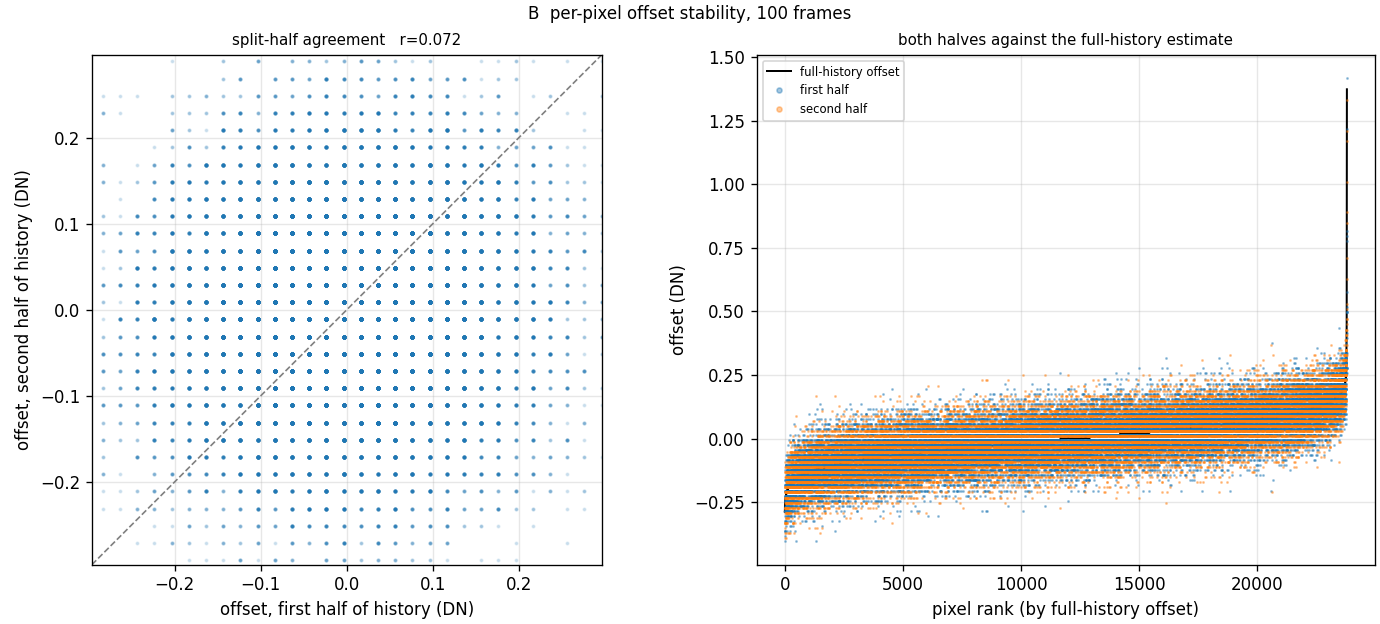
\includegraphics[width=\linewidth]{dark-signals-stability}
\caption{Split-half reliability of the per-pixel offset, $n = 100$ frames
split $50/50$ by time. Left: first-half offset vs.\ second-half offset,
per pixel; the dashed line is the identity. Right: both halves and the
full-history estimate, all sorted by the full-history offset.}
\label{fig:stability}
\end{figure}

%======================================================================
\section{Does the dark level drift with time?}
\label{sec:temporal}
%======================================================================

\paragraph{Why we asked this.}
Three timescales are relevant to how a dark correction is actually applied
in practice: seconds, within one archive's own batch of dark frames;
minutes, between a dark batch and the lit frames it corrects, within the
same archive; and anywhere from minutes to days, between different
archives. If $\mu(k)$ drifts meaningfully on any of these scales, a dark
frame taken at the wrong time is a source of error even if every pixel's
$p_i$ is estimated perfectly.

\paragraph{What we did.}
For each timescale, we regress the frame-level mean $\mu(k)$ against
elapsed time $t(k)$ (seconds within one archive for the short scale, real
wall-clock hours across archives for the long scale) by ordinary least
squares. With time centered, $t'(k) = t(k) - \bar t$, the least-squares
slope has the simple closed form
\[
\text{slope} = \frac{\sum_k t'(k)\,(\mu(k) - \bar\mu)}{\sum_k t'(k)^2}
= \frac{\mathrm{cov}(t, \mu)}{\mathrm{Var}(t)},
\]
i.e.\ the covariance between time and level, divided by the variance of
time alone. Significance is judged by a permutation test
(\S\ref{sec:notation}): shuffle the frame-level means against the fixed
time values $2000$ times, recompute the slope each time, and see where the
real slope falls among the shuffled ones. This sidesteps having to assume
the frame-mean residuals are themselves normally distributed, which is a
separate question from the one \S\ref{sec:normality} answers (that one
concerns the per-pixel offset, not the frame-to-frame level).
\code{dark\_temporal\_check(samps, ch)} implements both scales.

\emph{The middle timescale --- dark to lit, minutes, within one archive ---
could not be tested on this sample.} It requires two dark batches
bracketing the same lit sequence, and every archive here stores only one
(``after'') batch. This is exactly the gap that Decision~2
(\S\ref{sec:decisions}) closes going forward.

\emph{The long timescale needs one more precaution.} A ladder archive
(\code{C1017}, \code{C1018}) stores dark frames at 22 exposure times; a
single-rung archive stores only 8. Averaging each archive's \emph{entire}
set of dark frames to get one ``archive mean'' would silently compare
averages built from different mixes of exposures, confounding any real
drift with a difference in composition. We instead restrict the long-scale
comparison to the 8 exposure times common to every one of the nine
archives, so each archive's point in that comparison is built the same way.

\paragraph{What we found.}
Figure~\ref{fig:temporal} shows both scales. Within \code{C1017} (left),
the fitted slope is $+0.88\,\mathrm{DN}$ per $1000\,\mathrm{s}$, with a
permutation $p = 0.165$ --- not distinguishable from no trend at all across
an $11.5$-second dark batch. Between the nine archives (right), spanning
about 48 hours, the fitted slope is $+0.0001\,\mathrm{DN}$ per hour, $p =
0.333$ --- again consistent with no real drift once the comparison is
restricted to matched exposures. The right-hand panel does show a visible
sawtooth: the level jumps upward between \code{C1018} and \code{C1019},
and again between \code{C1022} and \code{C1023}, decaying gently downward
in between. Both jumps are small --- roughly $0.015$--$0.02\,\mathrm{DN}$,
about half of $\sigma_p$ (\S\ref{sec:estimator}) and two orders of
magnitude below the single-frame noise floor $\sigma_\varepsilon$ --- and
with only three apparent groupings in nine archives, there are far too few
repeats to say whether this is a real, repeatable effect (for instance, a
brief warm-up each time a capture session restarts) or simply what a
handful of points looks like under ordinary sampling variation. We record
it as an open question worth watching, not as a finding.

\begin{figure}[H]
\centering
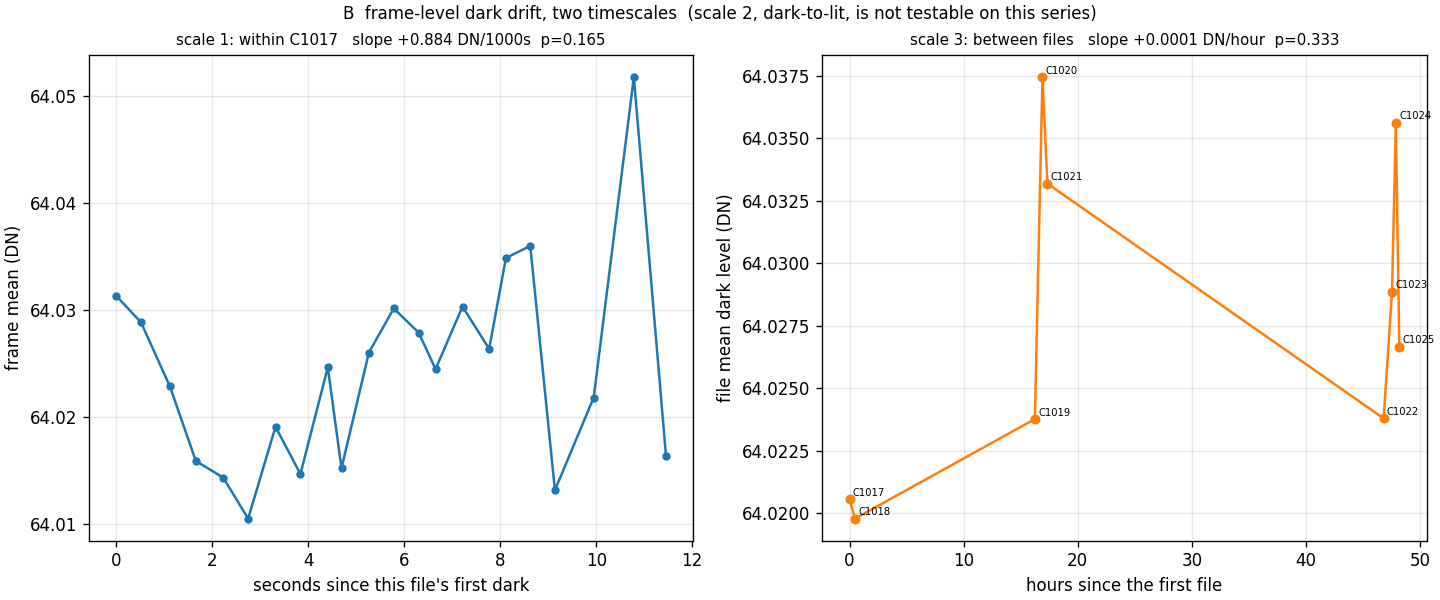
\includegraphics[width=\linewidth]{dark-signals-temporal}
\caption{Frame-level dark drift. Left: within one archive (\code{C1017}),
seconds. Right: between the nine archives, hours, restricted to the 8
exposure times common to all of them.}
\label{fig:temporal}
\end{figure}

%======================================================================
\section{Does the dark level, or its noise, depend on exposure duration?}
\label{sec:exposure}
%======================================================================

\paragraph{Why we asked this.}
This question has a direct, practical payoff: if the dark level (or its
noise) depends meaningfully on how long the exposure was, a whole ladder of
dark exposures is needed to correct every lit exposure correctly. If it
does not, a single dark exposure --- or a low one and a high one --- is
enough, freeing up capture time and storage.

\paragraph{A confound, faced directly.}
Within any one archive, the dark frames are captured in strictly increasing
exposure order, so \emph{elapsed time since the batch started} and
\emph{exposure duration} are the same variable, relabeled --- no test run
on one archive's own sequence can tell which of the two it is responding
to. They can only be told apart where the \emph{pairing} between exposure
time and elapsed time differs across archives, and it does: a ladder
archive visits 22 exposures over about 11.5 seconds; a single-rung archive
visits 8 of the same exposure values over a much shorter span, at different
relative positions in its own batch. Comparing many archives at the
\emph{same} exposure time, each having reached that exposure time at a
different point in its own batch, is the natural comparison this data set
offers. It is not a perfect one: it separates exposure duration from
absolute, cross-session time, but it does not fully separate exposure
duration from ``elapsed time since this particular archive's own dark
batch began,'' since every batch, regardless of how many exposures it
holds, proceeds shortest-exposure-first. This limitation is stated here
rather than glossed over, and the conclusion below is phrased with it in
mind.

\paragraph{What we did: one-way ANOVA with a permutation null.}
Treat exposure time as a factor with $G = 8$ levels (the common exposure
times), each represented by one frame from each of the 9 archives (so
$G=8$ groups of $9$ frames, $72$ frames total after restricting to the
common exposures). ``Analysis of variance'' asks whether the differences
\emph{between} the group means are large compared to the scatter
\emph{within} each group. Writing $y_{g,j}$ for the $j$-th frame's
statistic (mean or standard deviation) in exposure group $g$, $\bar y_g$
for that group's own mean, and $\bar y$ for the overall mean:
\[
\mathrm{SS}_{\mathrm{between}} = \sum_{g} n_g (\bar y_g - \bar y)^2, \qquad
\mathrm{SS}_{\mathrm{within}} = \sum_{g}\sum_{j} (y_{g,j} - \bar y_g)^2,
\]
with $n_g$ the number of frames in group $g$ (here, $9$ for every group).
Dividing each sum of squares by its degrees of freedom ($df_{\mathrm{between}}
= G - 1$, $df_{\mathrm{within}} = \sum_g n_g - G$) gives the two average
squared spreads being compared, and their ratio is the $F$-statistic:
\[
F = \frac{\mathrm{SS}_{\mathrm{between}}/df_{\mathrm{between}}}
         {\mathrm{SS}_{\mathrm{within}}/df_{\mathrm{within}}}.
\]
$F$ near $1$ means the between-group differences look like the same kind of
scatter already present within each group --- no real group effect; $F$
much larger than $1$ means the groups differ by more than their own
internal scatter would predict. Because the within-group counts here are
small (9 frames per group), we judge $F$ by a permutation test rather than
the textbook $F$-distribution: shuffle the exposure-time labels across all
72 frames (keeping the same group sizes), recompute $F$, $2000$ times, and
see where the real $F$ falls. This is implemented as
\code{dark\_exposure\_check(samps, ch, quantity)}, run once for the
per-frame mean (dark current, i.e.\ whether charge accumulates with
integration time) and once for the per-frame standard deviation (whether
the noise itself, as opposed to the level, depends on exposure).

\paragraph{What we found.}
For the level (Figure~\ref{fig:exposure-mean}): $F = 2.48$, permutation $p
= 0.026$ --- a real, statistically detectable effect, not attributable to
chance at the usual 5\% threshold. But the \emph{size} of that effect is
the more important number for the original question: the largest
difference between any two exposure groups' means is only
$0.0225\,\mathrm{DN}$, smaller than $\sigma_p$ itself
(\S\ref{sec:estimator}) and roughly $30$ times smaller than a single
frame's own noise, $\sigma_\varepsilon = 0.731\,\mathrm{DN}$. This is a
clean illustration of the distinction drawn in \S\ref{sec:notation}
between statistical and practical significance: the effect is real enough
to detect with $72$ frames, and yet far too small to be worth correcting
for in a subtraction that is already carrying three-tenths of a DN of
irreducible frame-to-frame noise. Given the acknowledged residual confound
with elapsed-time-since-batch-start, we do not claim this small effect is
purely an exposure-duration effect in the strict sense --- only that
whatever it is, it is too small to matter operationally.

For the noise (Figure~\ref{fig:exposure-std}): $F = 0.56$, permutation $p =
0.790$ --- no detectable effect at all; the per-frame standard deviation
does not depend on exposure duration in this data.

\begin{figure}[H]
\centering
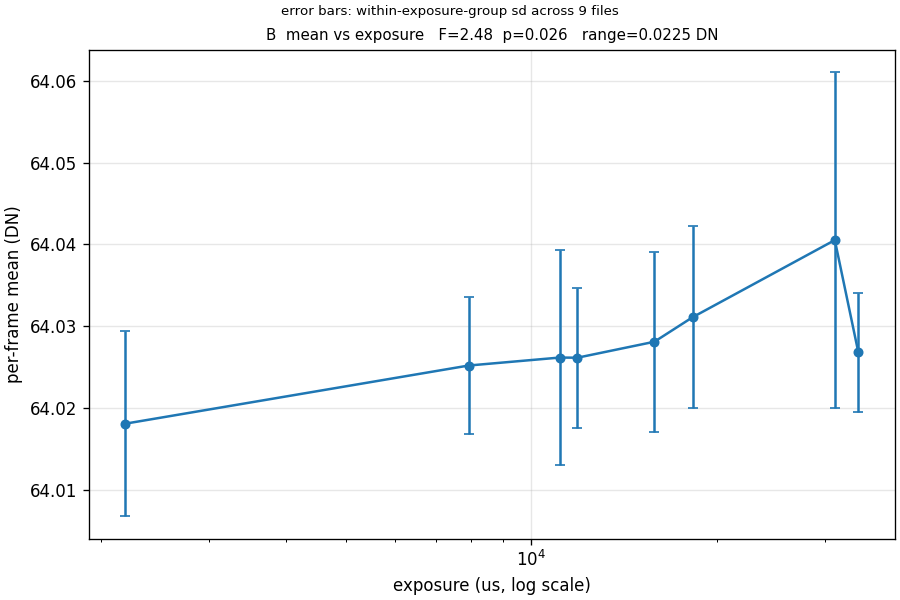
\includegraphics[width=0.85\linewidth]{dark-signals-exposure-mean}
\caption{Per-frame mean dark level vs.\ exposure time, restricted to the 8
exposure times common to all nine archives. Error bars are the
within-exposure-group standard deviation across archives.}
\label{fig:exposure-mean}
\end{figure}

\begin{figure}[H]
\centering
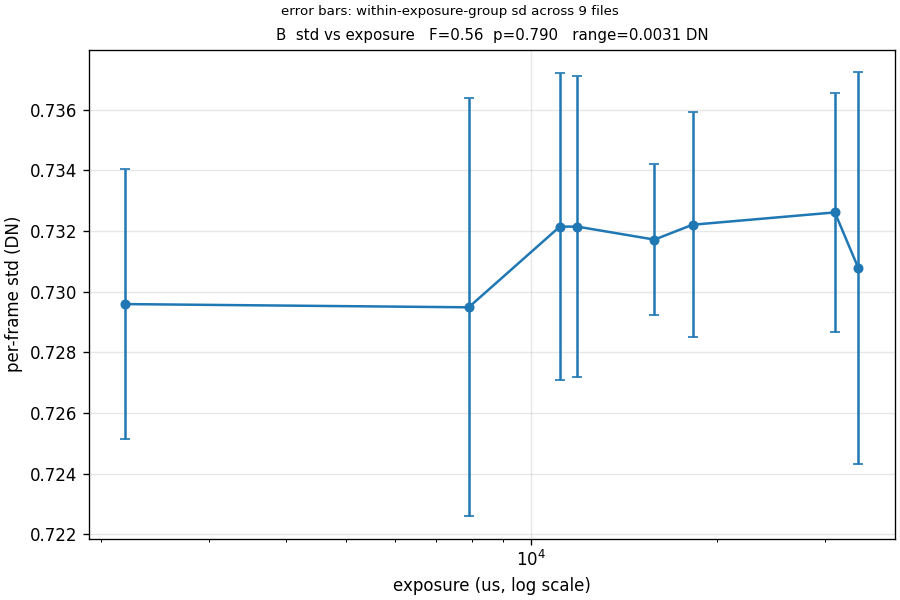
\includegraphics[width=0.85\linewidth]{dark-signals-exposure-std}
\caption{Per-frame standard deviation vs.\ exposure time, same restriction
as Figure~\ref{fig:exposure-mean}.}
\label{fig:exposure-std}
\end{figure}

%======================================================================
\section{Combining it all: the best per-pixel dark estimator}
\label{sec:estimator}
%======================================================================

\paragraph{Why we asked this.}
Everything above answers a piece of the puzzle. This section puts the
pieces together into an actual answer to the practical question: given a
new lit frame, what should be subtracted from it, pixel by pixel?

\paragraph{Restating the model with what we now know.}
Recall Equation~\ref{eq:model}, $d_i(k) = \mu(k) + p_i + \varepsilon_i(k)$.
We now know: $\mu(k)$ can be measured directly and freshly for any new dark
frame, with negligible sampling error of its own (it is already an average
over all $23{,}790$ pixels of one frame); its drift over the timescales we
could test is not detectably different from zero (\S\ref{sec:temporal}); it
does not detectably depend on exposure duration by an amount that matters
(\S\ref{sec:exposure}). $p_i$ is mostly indistinguishable from noise for a
typical pixel, but real and reproducible for a small population of hot
pixels (\S\ref{sec:stability}). $\varepsilon_i(k)$ is fresh, independent
noise that cannot be predicted for any specific future frame, by
construction.

\paragraph{An important, easy-to-miss point about what ``best'' means here.}
No procedure, however good, can predict $\varepsilon_i(k_{\mathrm{new}})$
--- the specific noise realization affecting a future lit frame's own dark
contribution --- because it is a fresh, independent draw that no
measurement taken at another time could ever have observed. That is not a
limitation of the estimator; it is a limitation of the physical situation.
The best any estimator can do is hit the \emph{predictable} part of the
dark signal, $\mu(k_{\mathrm{new}}) + p_i$ --- its expected value averaged
over that unavoidable fresh noise. Every comparison below therefore judges
candidate estimators by how close they come to $\mu(k_{\mathrm{new}}) +
p_i$, not by pretending to explain away noise nothing could explain away.

\paragraph{Estimating $p_i$ from history: the shrinkage estimator.}
$p_i$ is never observed by itself, only mixed with fresh noise,
$d_i(k) - \mu(k) = p_i + \varepsilon_i(k)$. Averaging this quantity over
$n$ historic frames for one pixel gives
\[
r_i = \frac{1}{n}\sum_{k=1}^n \big(d_i(k) - \mu(k)\big)
= p_i + \frac{1}{n}\sum_{k=1}^n \varepsilon_i(k),
\]
an unbiased estimate of $p_i$ whose own sampling variance is
$\mathrm{Var}(r_i) = \sigma_\varepsilon^2 / n$ (averaging $n$ independent
noise draws divides variance by $n$). If, in addition, the true
pixel-to-pixel spread of $p_i$ itself, $\sigma_p^2$, is known, there is a
simple, elementary way to combine the two pieces of information we have
about this one pixel's $p_i$: a working assumption that a typical pixel's
offset is near zero, with ``precision'' (inverse variance) $1/\sigma_p^2$;
and the specific measurement $r_i$ for this pixel, with precision
$n/\sigma_\varepsilon^2$. The minimum-variance way to combine two
independent, unbiased pieces of information about the same unknown is to
weight each by its own precision and renormalize. Doing that here gives
\begin{equation}
B = \frac{\sigma_p^2}{\sigma_p^2 + \sigma_\varepsilon^2/n}, \qquad
\hat p_i = B \, r_i, \qquad 0 \le B \le 1.
\label{eq:shrinkage}
\end{equation}
(Readers familiar with Bayesian statistics will recognize this as the
posterior mean of the standard normal-normal conjugate update; it is
derived here from ordinary variance arithmetic because nothing more is
needed.) $B$ close to $1$ means a pixel's own history is trustworthy and a
fresh single dark frame would add little beyond it; $B$ close to $0$ means
the apparent pixel-to-pixel spread is mostly sampling noise, and the
population average --- effectively, ignoring $p_i$ altogether --- is the
better bet.

\paragraph{Estimating the two variances from the data, not assuming them.}
$\sigma_\varepsilon^2$ is the leftover spread of $\varepsilon_i(k)$ once
both $\mu(k)$ and $r_i$ are removed, averaged over pixels:
$\sigma_\varepsilon^2 = \frac{1}{N_{\mathrm{px}}}\sum_i
\mathrm{Var}_k\big(d_i(k) - \mu(k) - r_i\big)$; this should sit close to
the single-frame standard deviation already seen in
Figure~\ref{fig:single-frame}. $\sigma_p^2$ is trickier, because the raw
spread of $r_i$ \emph{overstates} it: $\mathrm{Var}(r_i)$ mixes the real
between-pixel spread with $r_i$'s own sampling noise, $\sigma_p^2 +
\sigma_\varepsilon^2/n$ (this is the same ``total variance splits into a
real part and a sampling-noise part'' idea used throughout, and is the same
decomposition a random-effects ANOVA performs, with pixel playing the role
of ``group''; $B$ above is that decomposition's intraclass correlation).
Removing the known sampling-noise contribution gives the corrected estimate
\[
\sigma_p^2 = \max\!\big(\mathrm{Var}(r_i) - \sigma_\varepsilon^2/n,\; 0\big),
\]
clipped at zero because a negative raw result simply means the apparent
pixel-to-pixel spread is no larger than sampling noise predicts on its own
--- there is no fixed pattern left to estimate. Both quantities, together
with $B$, are computed by \code{estimate\_dark\_offset(samps, ch)}. On the
nine-archive pool: $\sigma_\varepsilon = 0.731\,\mathrm{DN}$, $\sigma_p =
0.028\,\mathrm{DN}$, $B = 0.131$ at $n = 100$.

\paragraph{Four candidate estimators, compared.}
With $\mu_{\mathrm{new}}$ standing for a freshly measured dark frame's own
spatial mean, we compare four ways of predicting
$\mu_{\mathrm{new}} + p_i$ for a future lit frame:

\begin{description}[leftmargin=2.7cm,style=nextline]
\item[A --- frame mean only] $\hat d_i = \mu_{\mathrm{new}}$, applied
  uniformly to every pixel (i.e.\ assume $p_i = 0$). Its error against the
  target is simply $p_i$ itself, so its root-mean-square error over all
  pixels is $\sigma_p$.
\item[B --- raw pooled history] $\hat d_i = \mu_{\mathrm{new}} + r_i$,
  using the plain historic average with no shrinkage. Its error is
  $-\frac1n\sum_k\varepsilon_i(k)$, RMS $= \sigma_\varepsilon/\sqrt n$.
\item[C --- shrunk pooled history] $\hat d_i = \mu_{\mathrm{new}} + B r_i$,
  Equation~\ref{eq:shrinkage}. A short calculation (expand $p_i - B r_i =
  (1-B)p_i - B\cdot\frac1n\sum_k\varepsilon_i(k)$, take the variance of both
  independent terms, and substitute $B$'s definition) gives mean-squared
  error exactly $(1-B)\,\sigma_p^2$, so RMS $= \sqrt{(1-B)}\,\sigma_p$ ---
  always at least as good as A, by construction.
\item[D --- today's practice] $\hat d_i = d_i(k_{\mathrm{match}})$: subtract
  one specific historic dark frame's own raw per-pixel value, implicitly
  treating its $\mu(k_{\mathrm{match}})$ as a stand-in for
  $\mu_{\mathrm{new}}$. Its error against the target is
  $\varepsilon_i(k_{\mathrm{match}})$ (plus any real difference between
  $\mu(k_{\mathrm{match}})$ and $\mu_{\mathrm{new}}$, which
  \S\ref{sec:temporal} found not to be detectably different from zero), so
  RMS $= \sigma_\varepsilon$.
\end{description}

\begin{table}[H]
\centering
\caption{The four estimators, evaluated with the numbers measured on this
sample ($\sigma_\varepsilon = 0.731\,\mathrm{DN}$, $\sigma_p =
0.028\,\mathrm{DN}$, $n = 100$, $B = 0.131$).}
\label{tab:estimators}
\begin{tabular}{@{}llll@{}}
\toprule
Estimator & What it subtracts & RMS error formula & RMS error (DN) \\
\midrule
A --- frame mean & $\mu_{\mathrm{new}}$ & $\sigma_p$ & $0.028$ \\
B --- raw pooled history & $\mu_{\mathrm{new}} + r_i$ & $\sigma_\varepsilon/\sqrt n$ & $0.073$ \\
C --- shrunk pooled history & $\mu_{\mathrm{new}} + B r_i$ & $\sqrt{1-B}\,\sigma_p$ & $0.027$ \\
D --- today's practice & $d_i(k_{\mathrm{match}})$ & $\sigma_\varepsilon$ & $0.731$ \\
\bottomrule
\end{tabular}
\end{table}

\paragraph{What this means.}
Two results stand out. First, C improves on A by only about $7\%$
($0.027$ vs.\ $0.028\,\mathrm{DN}$) --- exactly what a small $B$ predicts,
and confirmation that chasing a fully pooled per-pixel history is not worth
the added bookkeeping for an ordinary pixel. Second, and by far the larger
finding: A beats D, today's actual practice, by a factor of about
$26$ in RMS error ($0.028$ vs.\ $0.731\,\mathrm{DN}$). Subtracting one
matched historic dark frame's own raw pixel values --- which feels like the
more careful, ``use the real measurement'' choice --- is in fact
dramatically worse than simply subtracting that frame's spatial average
uniformly, because it needlessly imports that one frame's entire share of
fresh, unpredictable noise, $\sigma_\varepsilon$, in place of the far
smaller, genuinely predictable quantity, $\sigma_p$. (For completeness: A
would lose to B, the raw pooled history, only once $n$ exceeds
$\sigma_\varepsilon^2/\sigma_p^2 \approx 662$ historic frames --- far more
than are presently collected for any one pixel.)

\paragraph{The exception: hot pixels.}
This ranking is for a \emph{typical} pixel, where $p_i$ is small and mostly
indistinguishable from noise. \S\ref{sec:stability} identified a small,
reproducible population where that is not true.
\code{estimate\_dark\_offset} flags these automatically: a pixel is marked
an outlier when its historic residual $r_i$ exceeds five times $r_i$'s own
predictive spread, $\sqrt{\sigma_p^2 + \sigma_\varepsilon^2/n}$ --- the full
uncertainty an ordinary pixel's $r_i$ can carry, sampling noise included,
rather than $\sigma_p$ alone. (An earlier version of this check compared
against $\sigma_p$ alone and flagged $1{,}589$ of $23{,}790$ pixels ---
clearly wrong, since it was penalizing ordinary pixels for $r_i$'s own
sampling noise, not for anything peculiar to the pixel. Correcting the
comparison brought the count down to a small, plausible number.) On this
sample, $12$ pixels out of $23{,}790$ are flagged this way, with offsets
from $0.4$ to $1.4\,\mathrm{DN}$ --- large enough, and reproducible enough
(\S\ref{sec:stability}), that estimator A's flat assumption $p_i = 0$
leaves a real, avoidable bias at exactly these locations. For this small
list, estimator C (or D) is the better choice; for everywhere else, A is.

%======================================================================
\section{Decisions}
\label{sec:decisions}
%======================================================================

Two concrete changes follow from the six tests above. Both are proposed,
not yet implemented, in \file{docs/design-updates-prompt-1.md}, which is
the place to look for the implementation plan, cost, and open questions;
this section states only the reasoning, which is what this document is
for.

\subsection*{Decision 1: subtract the fresh dark frame's spatial mean, not
its raw per-pixel array}

Everywhere except the identified hot pixels, \S\ref{sec:estimator} shows
that subtracting a freshly measured dark frame's own spatial average,
uniformly across every pixel, is about $26$ times more accurate (in RMS
error against the predictable part of the dark signal) than the present
practice of subtracting that one frame's raw pixel-by-pixel values. This
is because a frame mean, averaged over $23{,}790$ pixels, already carries
almost none of a single dark frame's own read noise, while a raw per-pixel
value carries all of it. For the small, explicitly identified set of hot
pixels, their own pooled historic correction (or a matched raw frame) should
still be used, since for them the fixed offset $p_i$ is real, sizeable, and
well estimated by history.

\subsection*{Decision 2: replace the exposure ladder with a before/after
pair}

\S\ref{sec:exposure} found no dark-level or noise dependence on exposure
duration large enough to matter operationally: the detectable effect on
level is about $30$ times smaller than a single frame's own noise. This
means a full ladder of dark exposures, one per exposure time used in the
lit sweep, is not needed for accuracy. What \emph{does} matter, per
Decision~1, is having a good, fresh estimate of $\mu(k)$ close in time to
the lit frames it will correct --- and \S\ref{sec:temporal} could not test
the one timescale that matters most for that (dark-to-lit, within one
sweep), because every archive in this sample keeps only a single
(``after'') dark batch. Reinstating a ``before'' batch as well as an
``after'' batch, bracketing both the pre-image sweep and the measurement
sweep, closes that gap directly: it gives two independent, closely-timed
estimates of $\mu(k)$ to average or compare, and, as a side benefit, makes
the previously untestable middle timescale testable for the first time.

%======================================================================
\section{Provenance and open items}
%======================================================================

\begin{itemize}
\item Code: \file{desktop/padanalysis/analysis\_2.py}, functions
  \code{dark\_analysis1}, \code{dark\_analysis2}, \code{dark\_cdf\_check},
  \code{dark\_stability\_check}, \code{dark\_temporal\_check},
  \code{dark\_exposure\_check}, \code{estimate\_dark\_offset},
  \code{predict\_dark}.
\item Sample set: \code{C1017}--\code{C1025}, measurement sweep, channel
  \code{B}, $100$ pooled dark frames.
\item Related documents: \file{docs/design-updates-prompt-1.md} (the
  implementation plan for both decisions above);
  \file{docs/reference\_framework\_preimage\_and\_chips.md} (the earlier,
  pre-2026-08 finding that dark-frame spatial structure is negligible, on
  archives that did keep before/after pairs); \file{tex/R\_inf\_guide.tex}
  (where \code{sig = lit - dark} enters the larger photometric chain).
\item Open items, not yet acted on: everything above is channel \code{B}
  only --- \code{R}, \code{Gr}, and \code{Gb} have not been run through
  this same battery of tests; the apparent session-boundary step pattern in
  Figure~\ref{fig:temporal} is unconfirmed, with only three groupings
  observed; and both decisions in \S\ref{sec:decisions} remain proposals
  until implemented and re-validated on data captured under the new
  protocol.
\end{itemize}

\end{document}
